% !TeX spellcheck = en_US
% !TeX root = main.tex

\section{Navigation and Organisation}
\subsection{Card Sorting}
% Reflect on the success of the Card Sorting design activity you did in Week 4
% Include the testing plan you developed for the activity
% Include photos you took of the activity running
% What feedback did you get and how did it inform your early content organisation decisions?
% Which organisation systems will you use in your website and why?

\subsubsection{The Plan}
To begin there were three main areas of content were identified: Git Reference Summary, Main storyline/tutorial, Interactive Quiz. These areas were then assigned a rank and associated keywords:
\begin{itemize}
	\item\textbf{Git Reference Summary}
	\begin{itemize}
		\item Shows all the commands and a basic overview of what they do
		\item This will be visited most by people coming back because they forgot something or wanted to know more outside of the main storyline
		\item \textbf{Rank:} 2
		\item \textbf{Keywords:} Advanced, Reflection, Quick
	\end{itemize}
	\item\textbf{Main storyline/tutorial}
	\begin{itemize}
		\item This will be most frequently visited by new comers and people just visiting the site
		\item \textbf{Rank:} 1
		\item \textbf{Keywords:} Beginner, Interesting, Interactive
	\end{itemize}
	\item\textbf{Interactive Quiz}
	\begin{itemize}
		\item Some of this will also be embedded inside the storyline
		\item People wanting a challenge and to learn more
		\item \textbf{Rank:} 3
		\item \textbf{Keywords:} Self Learning, Interactive, All Levels
	\end{itemize}	
\end{itemize}

For this survey I chose to go with an Open Card Sort because I wanted to observe how they thought about grouping and what is easier or more important to sort before arriving at a final decision. After the users had finished with sorting the cards, a couple of follow up questions/discussions would be had around why they named the groups they did.

\subsubsection{Execution}
In order to execute the card sorting, Trello was used for the physical moving of cards around. This decision was made because it best allows people to move the cards around like they would physically, while still providing them with the easy of changing the names of the groups.

\subsubsection{Results}
\begin{note}{Person 1}
	\begin{figure}[H]
		\centering
		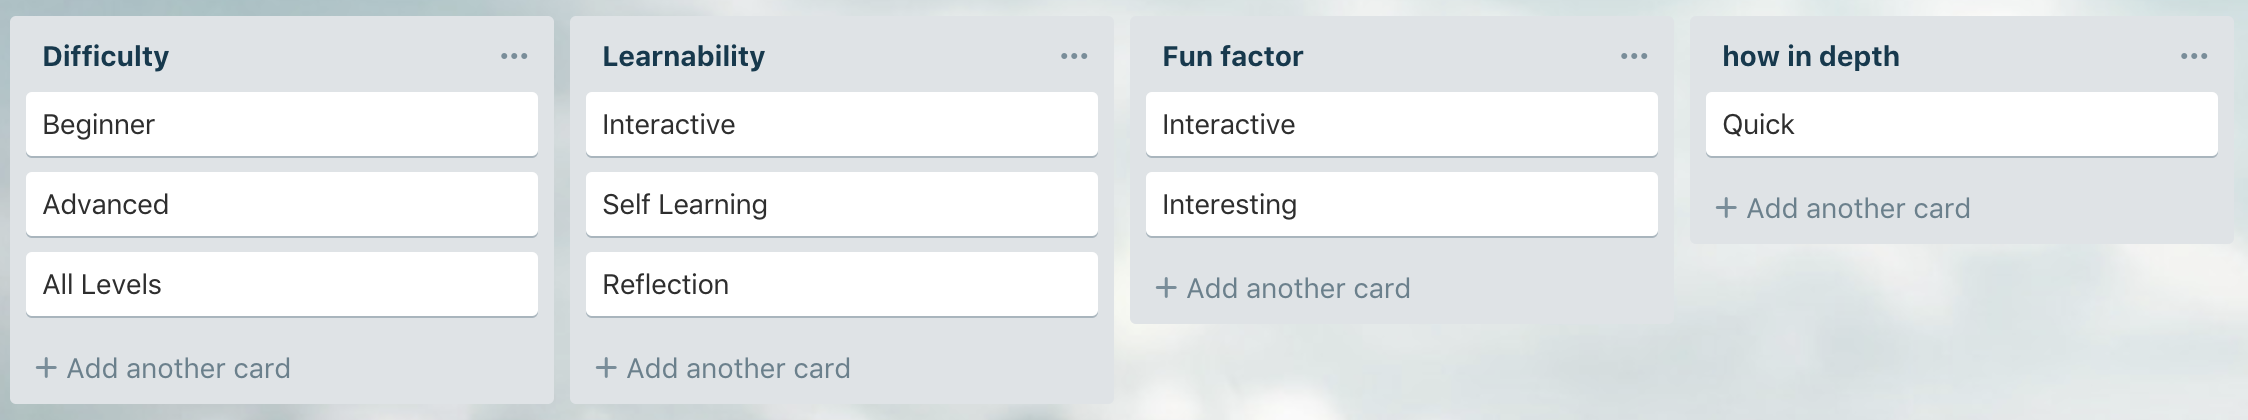
\includegraphics[width=\linewidth]{card1}	
		\caption{Person 1's Card Sorting Result}
	\end{figure}

	How did you group the tags?
	\begin{leftbar}
		Beginner and advanced are varying difficulties, I don't know if that is something I can choose. All levels are associated, can I filter by difficulty level on the side.\\\\
		Grouped them because the concepts are the same, but on the site I wouldn't expect beginner and advance to be together.
	\end{leftbar}

	How did you name the groups?
	\begin{leftbar}
		\begin{itemize}
			\item Difficulty
			\begin{itemize}
				\item When you play a video game you pick your difficulty level
			\end{itemize}
			\item Learnability
			\begin{itemize}
				\item Self learning, learnability makes sense
				\item Interactive is key to learning
				\item Reflection is key to learning, gauge how successful you were
			\end{itemize}
			\item Fun Factor
			\begin{itemize}
				\item Interactive website's are fun, reading a static page can be quite passive and boring
				\item It's interesting because I am curious and it feels more tactile
			\end{itemize}
			\item How in Depth (\textit{mean not very in depth})	
			\begin{itemize}
				\item I would go through the site really quickly
				\item So the level of detail in the website is probably really shallow
			\end{itemize}
		\end{itemize}
	\end{leftbar}
\end{note}

\begin{note}{Person 2}
	\begin{figure}[H]
		\centering
		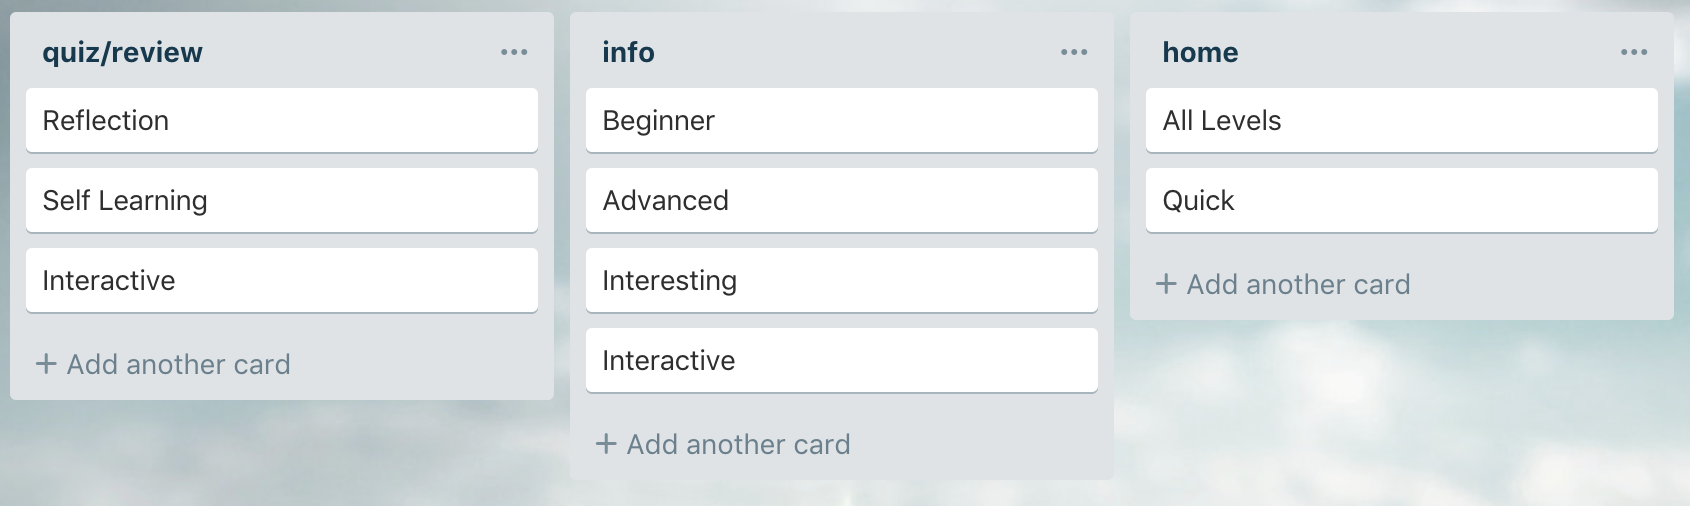
\includegraphics[width=\linewidth]{card2}	
		\caption{Person 2's Card Sorting Result}
	\end{figure}

	How did you group the tags?
	\begin{leftbar}
		Beginner and advanced are linked and interesting is cool\\\\
		All Levels and Quick are navigation type\\\\
		Reflection/SL/Interactive seem like quizzing	
	\end{leftbar}
	
	How did you name the groups?
	\begin{leftbar}
		\begin{itemize}
			\item Quiz/Review
			\begin{itemize}
				\item Reflection/SL is like looking back at what you learnt
				\item Looking back
			\end{itemize}
			\item Info
			\begin{itemize}
				\item Looking at Beginner and Advanced and interactive is like the middle of where you go
				\item Middle man of the navigation
			\end{itemize}
			\item Home
			\begin{itemize}
				\item They seem like navigation and be able to go through the site
			\end{itemize}
		\end{itemize}
	\end{leftbar}
\end{note}



\subsection{Navigation Systems}
% What were the key things you learned from your Navigation Systems group discussion?
% Write a brief response of your own to the guiding questions for this group discussion
% Which navigation systems will you use in your website and why?
A lot of the shown ``correct'' styles of navigation systems followed a similar style and placement. A lot of incorrect styles were outside the norm of having common elements. These elements are:
\begin{itemize}
	\item A main banner which include a general logo and quick navigation links underneath
	\item Most of the examples also used an inner page navigation panel on the left for filtering content on the current page	
\end{itemize}
Reflecting on the themes and the presentation styles used across websites that are considered good design, a similar layout will be used for this website. However slight modifications will be made to suit a scrolling storyline layout. To increase screen size and make the website appear more story like, the main logo will be reduced to be inline with the primary navigation menu. A side navigation menu will be created but it will be semi-hidden for a majority of the website and only showing itself when the mouse interacts with the shown tip.


\subsection{Site Map}
% Draw a site map that visualises the navigation flow of your website
% Include any internal (between pages) and external links
% Storyboard how one of your personas will navigate your website

\subsection{Visual Organisation}
% What were the key things you learned from you Visual Organisation group discussion?
% Write a brief response of your own to the guiding questions for this group discussion

\subsection{Interactivity and Functionality}
% Draw wireframes for each type of page in your website (i.e. if you have 5 pages that function very similarly, you only need to draw 1 wireframe)
% These can be derived from the same mockups you produced for Paper Prototyping
% Add annotations to describe:
% - how each interactive element functions
% - how they are designed to engage your specific target audience
% - how they are designed to strengthen the educational content
% - and how you think it will be implemented at this stage (HTML, CSS or JavaScript)

\subsection{Paper Prototyping}
% Reflect on the success of the Paper Prototyping design activity you did in Week 6
% Include photos/screenshots of your paper prototypes
% Include the testing plan you developed for the activity
% Include photos you took of the activity running
% What feedback did you get and how did it inform your visual organisation, navigation and functionality decisions?
\todo[inline]{Include Photo here}
The paper prototype was broken up into the following tests:

\subsubsection{Learn the Basics}
\begin{itemize}
	\item\textbf{Do:} ``Learn the basics''
	\item\textbf{Watch:} If they scroll through the homepage or jump to references
	\begin{itemize}
		\item\textbf{Person 1:} Hovered over the code snippet. Hovered over the heading. ``Will I be looking at whitespace''
	\end{itemize}
	\item\textbf{Ask:}
	\begin{itemize}
		\item ``Was it initiative to scroll	the page?''
		\begin{itemize}
			\item\textbf{Person 1:} Yeah very initiative, but there is no menu have to scan the entire page
		\end{itemize}
		\item ``Do you feel like the content is will spaced out?''
		\begin{itemize}
			\item\textbf{Person 1:} Yeah but vertical spacing is verging on a little too much
		\end{itemize}
	\end{itemize}
\end{itemize}


\subsubsection{Complete the Quiz}
\begin{itemize}
	\item\textbf{Do:} ``Complete the Quiz''
	\item\textbf{Watch:} How capable each of the controls in the quiz are
	\begin{itemize}
		\item\textbf{Person 1:} Got really confused about the terminal thing
	\end{itemize}
	\item\textbf{Ask:}
	\begin{itemize}
		\item ``Did you feel like it was obvious there was a quiz?''
		\begin{itemize}
			\item\textbf{Person 1:} Yeah it was obvious because of the quiz button. Weird it was between references and about
		\end{itemize}
		\item ``Was the Quiz easy to flow through?''
		\begin{itemize}
			\item\textbf{Person 1:} I don't know how many questions there are... Yes
		\end{itemize}
		\item ``Do you think you would benefit from the quiz?''
		\begin{itemize}
			\item\textbf{Person 1:} Yes cause I know what I don't know, find out weak spots
		\end{itemize}
	\end{itemize}	
\end{itemize}


\subsubsection{Get information on Advanced commands}
\begin{itemize}
	\item\textbf{Do:} ``Get information on Advanced commands''
	\item\textbf{Watch:} If they scroll through the home page screen first or go straight to the references page
	\begin{itemize}
		\item\textbf{Person 1:} Went to the homepage first
	\end{itemize}
	\item\textbf{Ask:}
	\begin{itemize}
		\item ``Was it clear that there is a references overview page?''
		\begin{itemize}
			\item\textbf{Person 1:} Yeah but I thought it was citations, not git command references
		\end{itemize}
	\end{itemize}	
\end{itemize}


\subsubsection{View information about the creator}
\begin{itemize}
	\item\textbf{Do:} ``View information about the site creator''
	\item\textbf{Watch:} How easy the navigation bar is to use
	\item\textbf{Ask:}
	\begin{itemize}
		\item ``Did you know exactly where you wanted to go?''
		\begin{itemize}
			\item\textbf{Person 1:} yeah but thought about was about the page not about the person
		\end{itemize}
	\end{itemize}	
\end{itemize}


\subsubsection{How do you update your git?}
\begin{itemize}
	\item\textbf{Do:} ``How do you update your git repo?''
	\item\textbf{Watch:} If they navigate to the references or the home page
	\item\textbf{Ask:}
	\begin{itemize}
		\item ``Did you know where you needed to go?''
		\begin{itemize}
			\item\textbf{Person 1:} Yeah I had a vague idea because I started on that page. I wouldn't if I didn't scroll the page
		\end{itemize}
	\end{itemize}	
\end{itemize}
